\documentclass[11pt]{article}
\usepackage[utf8]{inputenc}
\usepackage{amsmath}
\usepackage{amsfonts}
\usepackage{amssymb}
\usepackage{graphicx}
\usepackage{float}
\usepackage{hyperref}

\usepackage{todonotes}

\usepackage{rsfso} %Add the fancy L used in lagrange
\usepackage{siunitx}

\newcommand{\thomas}[1]{\todo[inline,color=black!30]{Thomas: #1}}
\newcommand{\mikkel}[1]{\todo[inline,linecolor=green!100,backgroundcolor=red!70, bordercolor=green]{Mikkel: #1}}

%Information to be included in the title page:
\title{Real-Time Systems}
\author{Thomas S. Christensen, Mikkel Skaarup Jaedicke}
\date{Jan, 2017}

\begin{document}
%!TEX root = ../main.tex

\section{Test Bed}
A simple setup for testing pendulum systems will be devised.
This will assist in better understanding the control problems facing the authors in creating a double pendulum control system.
During the process of building the setup, it is expected that some knowledge will be gained that will help in the design of the final system.
In order to properly design the test bed it is necessary to first determine what the expected outcome is from the testing.
Clearly, the goal is to rigorously determine the requirements of the full-scale system.
The requirements fall into a few categories:

\begin{itemize}
	\item \textbf{Mechanical:} The difficulty of the control is expected to be closely linked to the rigidity of the platform.
	In the ideal case, the cart will move only along one axis, say the x-axis.
	In the real case however, there is likely to be issues such as wobble along the remaining axes due to lack of rigidity in the drive mechanism.
	The test bed will allow a thorough investigation of the requirements appertaining these issues.
	\item \textbf{Electromechanical:} A number of electromechanical devices are required on the final platform: encoders, motors and switches.
	Using the test bed, experimentation can be done on the required resolution and sampling of encoders, the required speed of the motor in order to fulfil different control scenarios such as full swing-up or maintaining stability and finally, what switches are required, or desired, in the final system.
	\item \textbf{Control:} As previously mentioned, the real world is littered with inaccuracies which cannot reasonably be accounted for in simulations.
	While much of the design of the state space model and control scheme will be designed using a model, it is necessary to repeatedly verify the findings on a real system.
	While the test bed to be designed is unlikely to have the same characteristics as the full-scale system, it will provide the authors with experience in applying the control algorithms to a real system.
	The test bed should be able to, at least to some extent, perform the same manoeuvres as will be the case on the full-scale system.
	This includes maintaining stability of a pendulum in the upright position and performing a full swing-up of the pendulum.
\end{itemize}

Initially, the test bed is comprised of three parts, a drive mechanism, a cart and a pendulum with encoders.
These will be discussed in the subsequent sections.

\subsection{Drive Mechanism} % (fold)
\label{sub:drive_mechanism}
The drive mechanism is the part of the setup responsible for moving the cart.
Generally, what is required is a mechanism capable of creating linear motion.
In order to simplify the control as much as possible it would be desirable to use a low-backlash option such as a ball screw or lead screw setup.
These options are expensive and mechanically complicated to set up and while they may be under consideration for the full-scale system, this test bed will require something both simpler and cheaper.
Using a drive belt fitted to two wheels, one of which is driven by a small motor, will supply a simple, cost-effective method of creating motion.
The cart can then be attached to the belt which can be accelerated in either direction.
\\~\\
This option, clearly, is not as rigid as using a lead screw, as the cart is mounted on the belt.
Additionally, as the width of the platform increases, the slack in the belt will also increase.
Using a more narrow platform will increase the difficulty of performing the full swing-up, potentially increasing the difficulty of the control system.
An increased amount of slack due to the longer span of the belt will also impose a different set of control difficulties on the project.
This can be alleviated by mounting the cart on a set of rails using linear bearings, this will stabilise the platform and the belt be used only to drive the cart, rather than also supporting the weight of the cart.
\\~\\
A motor is necessary for driving the belt.
In order to perform the control, the motor has to be equipped with an encoder.
This will allow the system to have knowledge of the position of the cart relative to its starting position.

% subsection drive_mechanism (end)

\subsection{Cart} % (fold)
\label{sub:cart}
The cart holding the pendulum 
% subsection cart (end)

\subsection{Pendulum} % (fold)
\label{sub:pendulum}
The design of the pendulum requires that a few considerations are made.
Ideally, each pendulum would be a point-mass mounted using a rigid, mass-less bar.
As the creation of mass-less materials is beyond the scope of this report, an approximation will be made in an effort to simplify the mathematics required to model the system.
This means that the pendulum must be designed in such a way that the majority of the mass of the pendulum is centred around the pivot axis in one end of the pendulum.
It must be possible to determine the position of each link relative to the previous, therefore some type of encoder solution must be mounted at each joint.
Placing the encoder solution at the end of, and around the pivot axis of each pendulum will position the weight in the desired location.
The choice of the encoder solution is discussed further in the next section.

\subsection{Encoder} % (fold)
\label{sub:encoder}
As mentioned, it is necessary to know the position of each pendulum in order to fully control the system.
This can be accomplished using an encoder.
Generally, there are two types of encoders:
\begin{itemize}
	\item \textbf{Relative:} The position of the joint is known only relative to the starting position.
	In order for this scheme to be usable, some form of calibration is required such that the absolute position can be inferred based on the data given from the encoder.
	Any drift in the system will, over time, invalidate the calibration, meaning that in order to properly control the system, a new calibration is required.
	This can be avoided by including a tick at a certain, known position in the rotation.
	Based on the data given by the encoder it is possible to infer the velocity of a given joint at any time.
	\item \textbf{Absolute:} The position of the joint is known completely, regardless of starting position.
	While still allowing for the calculation of the velocity of a given joint, this encoder type also negates the necessity of a calibration.
\end{itemize}
The absolute encoder does provide benefits that the relative encoder does not.
When attempting to apply any sort of control to any type of plant, knowing the exact state of the output at any given point with known tolerance is very beneficial.
\\~\\
In addition to the function that the encoder provides, it should also conform to the physical constraints of the pendulum.
Due to the desire of creating the pendulum such that it, as closely as possible, resembles an ideal pendulum (massless rod with an attached point mass), it should be mounted as the joint at the end of the pendulum.
Additionally, a smaller design, while not necessary, would be preferable.
\\~\\
The remainder of this section will explore some of the options under consideration for this project.
\subsubsection{Encoder Disc, 3D Print} % (fold)
\label{ssub:encoder_wheel_3d_print}
In an effort to maintain low cost it is possible to 3D print an encoder disc.
An optical sensor is used to detect the rotation of the disc.
The resolution of the encoder is dictated by two factors: the size of the disc and the minimum feature size of the 3D printer.
By experiment, the smallest feature size which yields consistent results was found to be 0.75 mm.
An illustration of the encoder disc can be seen in figure \ref{fig:encoder_disc}.
For this solution to be practical the disc should be of limited size which in turn results in a lower resolution.
A trade-off must be made between resolution and size.
Size, especially, is a concern when mounting the encoders on each joint of the pendulums.
\\~\\
As mentioned, the holes in the disc can be detected using optical sensors.
Using just one optical sensor will allow only measuring the velocity.
In order to also detect the direction of travel it is necessary to introduce a second sensor.
By placing the two sensors out of phase, the direction of travel can be determined based on the order in which the rising edge of either sensors signal occurs.
By placing them 90\si{\degree} out of phase the pulses are generated equidistant and the effective resolution as created by the holes is doubled.
Mounting these sensors correctly is not a trivial task and may prove difficult.

%\begin{figure}[htbp]
%	\centering
	%\missingfigure
	%\includegraphics[width=0.95\textwidth]{}
	%\caption{A model of the encoder disc designed for use with the pendulum test bed.}
	%\label{fig:encoder_disc}
%\end{figure}

% subsubsection encoder_wheel_3d_print (end)
\subsubsection{Encoder Disc/Read Head, Procured} % (fold)
\label{ssub:encoder_disc_read_head_procured}
Many solutions exist already which are created specifically for reading the position of a rotating shaft or axle.
The cascaded pendulums are essentially rotating bodies connected by shafts, making many of these solutions applicable.
\\
One such solution is the HEDG-9000\cite{hedg9000} encoder disc and AEAT-9000-1GSH1\cite{aeat9000} read head combination.
The encoder disc provides 2048 counts per revolution, CPR.
% subsubsection encoder_disc_read_head_procured (end)

% subsection encoder (end)
% subsection pendulum (end)
\newpage
%!TEX root = ../main.tex

\section{Model Development} % (fold)
\label{sec:model_development}

In order to properly control the double pendulum it is necessary to develop a model of the system.
Throughout this section the model will be developed iteratively.
Initially including only the simple double pendulum, eventually including both friction and the cart.

\subsection{Simple Double Pendulum} % (fold)
\label{sub:simple_double_pendulum}
An illustration of the system can be seen in figure \ref{fig:doublependulum}.
As can be seen, the pendulums have masses $m_1$, $m_2$, suspended using rods of lengths $l_1$, $l_2$.
The rods are assumed to be massless.
The angles of the pendulums $\theta_1$, $\theta_2$, are measured as the offset from the stable position.
For convenience the two pendulums will be referred to as $p_1$ and $p_2$ where $p_2$ is suspended from $p_1$.

\begin{figure}
	\centering
	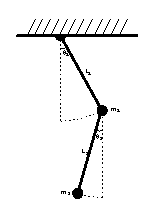
\includegraphics[width=.5\linewidth]{graphics/double_pendulum.eps}
	\caption{Illustration of the simple double pendulum.}
	\label{fig:doublependulum}
\end{figure}

Equations should be developed such that, given an initial state, the position and subsequent movement can be derived from them.
This can be achieved using the Euler-Lagrange differential equations.
These will be found for this system throughout the remainder of this section.
Firstly, the position of the pendulums as a function of the angle must be determined.
The pendulums are placed in the x-y plane with the origin placed at the point of suspension of $p_1$.
When the pendulums are in the stable position, $\theta_1=\theta_2=0$, they are aligned with the y-axis.
The x-axis is positive to the right of the stable position.
The coordinates of $p_1=(x_1,y_1)$ and $p_2=(x_2,y_2)$ are as follows:
\begin{align}
	x_1 &= l_1\sin{\theta_1}\\
	y_1 &= -l_1\cos{\theta_1}\\
	x_2 &= l_1\sin{\theta_1} + l_2\sin{\theta_2}\\
	y_2 &= -l_1\cos{\theta_1} - l_2\cos{\theta_2}
\end{align}
While the derivatives are not used until later, they are presented here for clarity:
\begin{align}
	\dot{x}_1 &= l_1\cos{\theta}_1\dot{\theta}_1\\
	\dot{y}_1 &= l_1\sin{\theta}_1\dot{\theta}_1\\
	\dot{x}_2 &= l_1\cos{\theta}_1\dot{\theta}_1 + l_2\cos{\theta_2}\dot{\theta}_2\\
	\dot{y}_2 &= l_1\sin{\theta}_1\dot{\theta}_1 + l_2\sin{\theta_2}\dot{\theta}_2
\end{align}
In order to calculate the Euler-Lagrange diff. eq. it is necessary to first determine the lagrangian, $\mathcal{l}$:
\begin{equation}
	\mathcal{L}=E_k-E_p
\end{equation}
Where $E_k$ is the kinetic energy of the system and $E_p$, the potential energy.
The derivation of $E_p$:
\begin{align}
	E_p &= m_1 g y_1 + m_2 g y_2\\
		&= -m_1 g l_1 \cos{\theta_1} - m_2 g l_1 \cos{\theta_1} - m_2 g l_2 \cos{\theta_2}\\
		&= -(m_1+m_2)l_1g \cos{\theta_1}-m_2 g l_2 \cos{\theta_2}
		\label{eq:ep}
\end{align}
The derivation of $E_k$:
\begin{equation}
	\label{eq:ek}
	E_k = \frac{1}{2}m_1v_1^2+\frac{1}{2}m_2v_2^2
\end{equation}
As movement is present along both axes, the total velocity of either pendulum can be found as the derivative of the position and Pythagoras:
\begin{align}
	v_1^2 &= \dot{x}_1^2+\dot{y}_1^2\\
		&= l_1^2\dot{\theta}_1^2\cos{\theta}_1^2+l_1^2\dot{\theta}_1^2\sin{\theta_1}^2\\
		&= (\cos{\theta_1}^2+\sin(\theta_1)^2)l_1^2\dot{\theta}_1
\end{align}
Using the Pythagorean identity:
\begin{equation}
	\label{eq:v1}
	v_1^2 = l_1^2\dot{\theta}_1^2
\end{equation}
Similarly:
\begin{align}
	v_2^2 &= \dot{x}_2^2+\dot{y}_2^2\\
	&= (l_1\cos{\theta}_1\dot{\theta}_1 + l_2\cos{\theta_2}\dot{\theta}_2)^2+(l_1\sin{\theta}_1\dot{\theta}_1 + l_2\sin{\theta_2}\dot{\theta}_2)^2\\
	\begin{split}
		&= l_1^2\dot\theta_1^2\cos{\theta_1}^2+l_2^2\dot\theta_2^2\cos{\theta_2}^2+2l_1l_2\dot\theta_1\dot\theta_2\cos{\theta_1}\cos{\theta_2}\\
		&\qquad +l_1^2\dot\theta_1^2\sin{\theta_1}^2+l_2^2\dot\theta_2\sin{\theta_2}+2l_1l_2\dot\theta_1\dot\theta_2\sin{\theta_1}\sin{\theta_2}
	\end{split}
\end{align}
Isolating cosine and sine from the terms pairwise, 1 and 4, 2 and 5, 3 and 6, yields:
\begin{align}
	\begin{split}
		v_2^2&=(\cos{\theta_1}^2+\sin{\theta_1}^2)l_1^2\dot\theta_1^2+(\cos{\theta_2}^2+\sin{\theta_2}^2)l_2^2\dot\theta_2^2\\
	&\qquad+(\cos{\theta_1}\cos{\theta_2}+\sin{\theta_1}\sin{\theta_2})2l_1l_2\dot\theta_1\dot\theta_2
	\end{split}
\end{align}
By applying the trigonimetric identities:
\begin{align}
	1&=\sin{\alpha^2}+\cos{\beta^2}\\
	\cos{(\alpha\pm\beta)}&=\cos\alpha\cos\beta\pm\sin\alpha\sin\beta
\end{align}
The result is found:
\begin{equation}
	\label{eq:v2}
	v_2^2=l_1^2\dot\theta_1^2+l_2^2\dot\theta_2^2+2l_1l_2\dot\theta_1^2\dot\theta_2^2\cos{(\theta_1-\theta_2)}
\end{equation}
Using equations \ref{eq:ep}, \ref{eq:ek}, \ref{eq:v1} and \ref{eq:v2} the lagrangian can be constructed:
\begin{align}
	\begin{split}
		\mathcal{L}&=\frac{1}{2}m_1l_1\dot\theta_1^2+\frac{1}{2}m_2\left(l_1^2\dot\theta_1^2+l_2^2\dot\theta_2^2+2l_1l_2\dot\theta_1^2\dot\theta_2^2\cos{(\theta_1-\theta_2)}\right)\\
		&\qquad+(m_1+m_2)l_1g\cos{\theta_1}+m_2l_2g\cos{\theta_2}
	\end{split}\\
	\begin{split}
		&=\frac{m_1l_1^2\dot\theta_1^2}{2}+\frac{m_2l_1^2\dot\theta_1^2}{2}+\frac{m_2l_2^2\dot\theta_2^2}{2}+l_1l_2\dot\theta_1^2\dot\theta_2^2\cos{(\theta_1-\theta_2)}\\
		&\qquad+(m_1+m_2)l_1g\cos{\theta_1}+m_2l_2g\cos{\theta_2}
	\end{split}
\end{align}
Which simplifies to:
\begin{equation}
	\label{eq:lagrangian}
	\mathcal{L}=\frac{(m_1+m_2)l_1^2\dot\theta_1^2}{2}+\frac{m_2l_2^2\dot\theta_2}{2}+(m_1+m_2)l_1g\cos{\theta_1}+m_2l_2g\cos{\theta_2}\\
\end{equation}
The Euler-Lagrange diff. eq. are defined as:
\begin{equation}
	\frac{d}{dt}\left(\frac{\partial \mathcal{L}}{\partial \dot\theta}\right)-\frac{\partial \mathcal{L}}{\partial \theta} = 0
\end{equation}
The three terms $\frac{\partial \mathcal{L}}{\partial \dot\theta}$,$\frac{d}{dt}\left(\frac{\partial \mathcal{L}}{\partial \dot\theta}\right)$ and $\frac{\partial l}{\partial \theta}$ are calculated next for each of the pendulums. For $p_1$:
\begin{align}
	\frac{\partial \mathcal{L}}{\partial \dot\theta_1}&=(m_1+m_2)l_1^2\dot\theta_1+m_2l_1l_2\dot\theta_2\cos{(\theta_1-\theta_2)}\\
	\begin{split}
		\frac{d}{dt}\left(\frac{\partial \mathcal{L}}{\partial \dot\theta_1}\right)&=(m_1+m_2)l_1^2\ddot\theta_1+m_2l_1l_2\ddot\theta_2\cos{(\theta_1-\theta_2)}\\
		&\qquad-m_2l_1l_2\dot\theta_2\sin{(\theta_1-\theta_2)(\dot\theta_1-\dot\theta_2)}
	\end{split}\\
	\frac{\partial \mathcal{L}}{\partial \theta_1} &= -m_2l_1l_2\dot\theta_1\dot\theta_2\sin(\theta_1-\theta_2)-(m_1+m_2)l_1g\sin{\theta_1}\\
	\begin{split}
		0&=(m_1+m_2)l_1\ddot\theta_1+m_2l_2\ddot\theta_2\cos{(\theta_1-\theta_2)}\\
		&\qquad+m_2l_2\dot\theta_2^2\sin{(\theta_1-\theta_2)}+(m_1+m_2)g\sin{\theta_1}
	\end{split}
\end{align}
And $p_2$:

\begin{align}
	\frac{\partial \mathcal{L}}{\partial \dot\theta_2}&=m_2l_2^2\dot\theta_2+m_2l_1l_2\dot\theta_1\cos{(\theta_1-\theta_2)}\\
	\begin{split}
		\frac{d}{dt}\left(\frac{\partial \mathcal{L}}{\partial \dot\theta_2}\right)&=m_2l_2^2\ddot\theta_2+m_2l_1l_2\ddot\theta_1\cos{(\theta_1-\theta_2)}\\
		&\qquad -m_2l_1l_2\dot\theta_1\sin{(\theta_1-\theta_2)}(\dot\theta_1-\dot\theta_2)
	\end{split}\\
	\frac{\partial \mathcal{L}}{\partial \theta_2} &=m_2l_1l_2\dot\theta_1\dot\theta_2\sin{(\theta_1-\theta_2)}-m_2l_2g\sin{\theta_2}\\
	\label{eq:part}
	\begin{split}
		0&=m_2l_2\ddot\theta_2+m_2l_1\ddot\theta_1\cos{(\theta_1-\theta_2)}\\
		&\qquad-m_2l_1\dot\theta_1^2\sin{(\theta_1-\theta_2)}+m_2g\sin{\theta_2}
	\end{split}
\end{align}
\thomas{eq. \ref{eq:part} has a minus in front of the first term according to our calculations. Determine why.}
% subsection simple_double_pendulum (end)

% section model_development (end)

\newpage
%!TEX root = main.tex
\begin{thebibliography}{21} %This number should be higher than the number of entries in the bibliography because reasons...
%	\bibitem{id}
%		Author(s) Last name, First name, Company/Organisation, Year. Full Title
\bibitem{hedg9000}
	Avago Technologies, August 2011, HEDG-9000 Series - Codewheel for use with Avago Technologies - Ultra-precision 17-Bit Absolute Single Turn Encoder
Encoder Modules AEAT-9000 series
\bibitem{aeat9000}
	Avago Technologies, April 2012, AEAT-9000-1GSH1 (Basic Option) - Ultra-precision 17-Bit Absolute Single Turn Encoder
\bibitem{mosfet}
	Infineon, August 2016, IPP045N10N3 Datasheet Rev. 2.8, \url{http://www.infineon.com/dgdl/Infineon-IPP045N10N3G-DS-v02_08-EN.pdf?fileId=db3a30431ce5fb52011d1e8b0cc31586}
\bibitem{bootstrap_ON}
	ON Semiconductor, December 2014, Design and Application Guide of Bootstrap Circuit forHigh-Voltage Gate-Drive IC, \url{https://www.fairchildsemi.com/application-notes/AN/AN-6076.pdf}
\bibitem{bootstrap_infineon}
	A. Merello, A. Rugginenti, M. Grasso, International Rectifier, Using Monolithic High Voltage Gate Drivers, \url{http://www.infineon.com/dgdl/Infineon-Using+Monolithci+Voltage+Gate+Drivers-UM-v01_00-EN.pdf?fileId=5546d462584d1d4a01585242c11947b1}
\bibitem{diode_ds}
	Surface Mount Ultrafast Rectifier, April 2014, \url{http://docs-europe.electrocomponents.com/webdocs/1405/0900766b81405c8a.pdf}
\bibitem{driver}
	Intersil, September 2015, HIP4081A Datasheet FN3659.8, \url{http://www.intersil.com/content/dam/Intersil/documents/hip4/hip4081a.pdf}
\end{thebibliography}
\end{document}